%% abtex2-modelo-relatorio-tecnico.tex, v-1.7.1 laurocesar
%% Copyright 2012-2013 by abnTeX2 group at http://abntex2.googlecode.com/ 
%%
%% This work may be distributed and/or modified under the
%% conditions of the LaTeX Project Public License, either version 1.3
%% of this license or (at your option) any later version.
%% The latest version of this license is in
%%   http://www.latex-project.org/lppl.txt
%% and version 1.3 or later is part of all distributions of LaTeX
%% version 2005/12/01 or later.
%%
%% This work has the LPPL maintenance status `maintained'.
%% 
%% The Current Maintainer of this work is the abnTeX2 team, led
%% by Lauro César Araujo. Further information are available on 
%% http://abntex2.googlecode.com/
%%
%% This work consists of the files abntex2-modelo-relatorio-tecnico.tex,
%% abntex2-modelo-include-comandos and abntex2-modelo-references.bib
%%

% ------------------------------------------------------------------------
% ------------------------------------------------------------------------
% abnTeX2: Modelo de Relatório Técnico/Acadêmico em conformidade com 
% ABNT NBR 10719:2011 Informação e documentação - Relatório técnico e/ou
% científico - Apresentação
% ------------------------------------------------------------------------ 
% ------------------------------------------------------------------------

% Alterado por Rodrigo Campiolo para apresentação de relatórios na disciplina
% de Redes de Computadores II do Bacharelado em Ciência da Computação da UTFPR-CM.


\documentclass[
    % -- opções da classe memoir --
    12pt,				% tamanho da fonte
    %openright,			% capítulos começam em pág ímpar (insere página vazia caso preciso)
    oneside,   	        % para impressão em verso e anverso use twoside. Oposto a oneside
    a4paper,			% tamanho do papel. 
    % -- opções da classe abntex2 --
    %chapter=TITLE,		% títulos de capítulos convertidos em letras maiúsculas
    %section=TITLE,		% títulos de seções convertidos em letras maiúsculas
    %subsection=TITLE,	% títulos de subseções convertidos em letras maiúsculas
    %subsubsection=TITLE,% títulos de subsubseções convertidos em letras maiúsculas
    % -- opções do pacote babel --
    english,			% idioma adicional para hifenização
    french,				% idioma adicional para hifenização
    spanish,			% idioma adicional para hifenização
    brazil,				% o último idioma é o principal do documento
    ]{pacotes/abntex2}


% ---
% PACOTES
% ---

% ---
% Pacotes fundamentais 
% ---
\usepackage{cmap}				% Mapear caracteres especiais no PDF
\usepackage{lmodern}			% Usa a fonte Latin Modern
\usepackage[T1]{fontenc}		% Selecao de codigos de fonte.
\usepackage[utf8]{inputenc}		% Codificacao do documento (conversão automática dos acentos)
\usepackage{indentfirst}		% Indenta o primeiro parágrafo de cada seção.
\usepackage{color}				% Controle das cores
\usepackage{graphicx}			% Inclusão de gráficos
% ---

% ---
% Pacotes adicionais, usados no anexo do modelo de folha de identificação
% ---
\usepackage{multicol}
\usepackage{multirow}
% ---
    
% ---
% Pacotes adicionais, usados apenas no âmbito do Modelo Canônico do abnteX2
% ---
\usepackage{lipsum}				% para geração de dummy text
% ---

% ---
% Pacotes de citações
% ---
\usepackage[brazilian,hyperpageref]{backref}	 % Paginas com as citações na bibl
\usepackage[alf]{pacotes/abntex2cite}	% Citações padrão ABNT
\usepackage{comment}
% ---

% ---
% Meus pacotes
% ---
\usepackage{float}
% ---

% --- 
% CONFIGURAÇÕES DE PACOTES
% --- 

% ---
% Configurações do pacote backref
% Usado sem a opção hyperpageref de backref
\renewcommand{\backrefpagesname}{Citado na(s) página(s):~}
% Texto padrão antes do número das páginas
\renewcommand{\backref}{}
% Define os textos da citação
\renewcommand*{\backrefalt}[4]{
    \ifcase #1 %
        Nenhuma citação no texto.%
    \or
        Citado na página #2.%
    \else
        Citado #1 vezes nas páginas #2.%
    \fi}%
% ---

% ---
% Informações de dados para CAPA e FOLHA DE ROSTO
% ---
\titulo{Implementação do Sistema de Arquivos FAT32}
\autor{João Victor Briganti\\Luiz Gustavo Takeda\\Matheus Floriano Saito}
\local{Campo Mourão}
\data{Fevereiro / 2025}
\instituicao{%
  Universidade Tecnológica Federal do Paraná -- UTFPR
  \par
  Departa           mento Acadêmico de Computação -- DACOM
  \par
  Bacharelado em Ciência da Computação -- BCC
}
\tipotrabalho{Relatório técnico}
% O preambulo deve conter o tipo do trabalho, o objetivo, 
% o nome da instituição e a área de concentração 
\preambulo{Relatório técnico de atividade prática solicitado pelo professor Rodrigo Campiolo na disciplina de Sistemas Operacionais do Bacharelado em Ciência da Computação da Universidade Tecnológica Federal do Paraná.}
% ---

% ---
% Configurações de aparência do PDF final

% alterando o aspecto da cor azul
\definecolor{blue}{RGB}{41,5,195}

% informações do PDF
\makeatletter
\hypersetup{
        %pagebackref=true,
        pdftitle={\@title}, 
        pdfauthor={\@author},
        pdfsubject={\imprimirpreambulo},
        pdfcreator={LaTeX with abnTeX2},
        pdfkeywords={abnt}{latex}{abntex}{abntex2}{relatório técnico}, 
        colorlinks=true,       		% false: boxed links; true: colored links
        linkcolor=blue,          	% color of internal links
        citecolor=blue,        		% color of links to bibliography
        filecolor=magenta,      		% color of file links
        urlcolor=blue,
        bookmarksdepth=4
}
\makeatother
% --- 

% --- 
% Espaçamentos entre linhas e parágrafos 
% --- 

% O tamanho do parágrafo é dado por:
\setlength{\parindent}{1.3cm}

% Controle do espaçamento entre um parágrafo e outro:
\setlength{\parskip}{0.2cm}  % tente também \onelineskip

% ---
% compila o indice
% ---
\makeindex
% ---

% Omite a numeração de capítulos
\renewcommand*\thesection{\arabic{section}}



% ----
% Início do documento
% ----
\begin{document}

% Retira espaço extra obsoleto entre as frases.
\frenchspacing 

% ----------------------------------------------------------
% ELEMENTOS PRÉ-TEXTUAIS
% ----------------------------------------------------------
% \pretextual

% ---
% Capa
% ---
%\imprimircapa
% ---

% ---
% Folha de rosto
% (o * indica que haverá a ficha bibliográfica)
% ---
\imprimirfolhaderosto
% ---


% ---
% RESUMO
% ---

% resumo na língua vernácula (obrigatório)
\begin{resumo}

Este estudo teve como objetivo investigar e implementar um sistema de arquivos FAT32 operando em uma imagem de disco em um sistema GNU/Linux. A implementação foi realizada em C++, utilizando uma abordagem modular que facilitou a organização e a manutenção do código. O estudo incluiu uma análise detalhada das estruturas do FAT32, com ênfase na manipulação de tabelas de alocação, entradas de diretório e clusters. Como resultado, o trabalho proporcionou uma compreensão aprofundada, tanto teórica quanto prática, sobre a implementação e o funcionamento do sistema de arquivos FAT32.

 \vspace{\onelineskip}
    
 \noindent
 \textbf{Palavras-chave}: C++; GNU/Linux; Imagem de Disco.
 
\end{resumo}% ---

% ---
% inserir lista de ilustrações
% ---
%\pdfbookmark[0]{\listfigurename}{lof}
%\listoffigures*
%\cleardoublepage
% ---

% ---
% inserir lista de tabelas
% ---
%\pdfbookmark[0]{\listtablename}{lot}
%\listoftables*
%\cleardoublepage
% ---

% ---
% inserir lista de abreviaturas e siglas
% ---
%\begin{siglas}
%  \item[IP] Internet Protocol
%  \item[TCP] Transmission Control Protocol
%  \item[UDP] User Datagram Protocol
%\end{siglas}
% ---

% ---
% inserir o sumario
% ---
\pdfbookmark[0]{\contentsname}{toc}
\tableofcontents*
\cleardoublepage
% ---

% ----------------------------------------------------------
% ELEMENTOS TEXTUAIS
% ----------------------------------------------------------
\textual

\makeatletter
\renewcommand{\chapter}{\@gobbletwo}
\makeatother

\section{Introdução}
\label{sec:introducao}

Um sistema de arquivos é uma parte fundamental de um sistema operacional, responsável por organizar, armazenar e gerenciar os dados de forma eficiente e confiável em dispositivos de armazenamento, como discos rígidos e SSDs. Este sistema  desempenha um papel crucial ao permitir que aplicativos e usuários armazenem informações que precisam ser acessadas e preservadas mesmo após o encerramento de um processo ou desligamento do computador~\cite{tanenbaum2016}.

FAT (File Allocation Table) é um sistema de arquivos desenvolvido no final de 1970. Originalmente utilizado no sistema operacional MS-DOS, o FAT evoluiu ao longo do tempo para suportar mídias maiores, resultando em três variantes principais: FAT12, FAT16 e FAT32. A principal diferença entre essas versões está no tamanho, em bits, das entradas na tabela de alocação, que variam de 12 a 32 bits~\cite{microsoft2000}.

\section{Objetivo}
\label{sec:objetivos}

O objetivo deste trabalho é compreender de forma aprofundada o funcionamento do sistema de arquivos FAT32. Busca-se explorar seus detalhes de implementação, incluindo a estrutura da tabela de alocação, a organização dos dados no disco e os mecanismos de gerenciamento de espaço.

\section{Fundamentação}
\label{sec:fundamentacao}

O sistema de arquivos é um componente essencial em qualquer sistema operacional, sendo responsável pela organização, armazenamento e recuperação de dados em dispositivos de armazenamento. Este sistema fornece uma abstração que permite ao usuário interagir com os dados de forma intuitiva, sem a necessidade de compreender os detalhes de baixo nível sobre a disposição física dos mesmos.

Como camada de abstração, o sistema de arquivos utiliza mecanismos como divisão em blocos/setores, estrutura hierárquica de diretórios, arquivos e metadados para ocultar a complexidade física do usuário. Os arquivos, que representam as unidades básicas de dados, são armazenados de maneira lógica e podem conter desde pequenos trechos de texto até grandes volumes de informações binárias, enquanto os diretórios organizam esses arquivos em uma árvore hierárquica, permitindo uma navegação intuitiva. Essa estrutura hierárquica também possibilita a criação de subdiretórios, facilitando a categorização e o gerenciamento de grandes volumes de dados.

Além disso, o sistema de arquivos fragmenta o armazenamento em blocos e os mapeia logicamente, criando uma representação unificada dos dados, independentemente de sua dispersão física no dispositivo. Os metadados desempenham um papel crítico nesse processo, armazenando informações como permissões de acesso, tamanho, localização física no disco e datas de modificação. Tabelas de alocação, por exemplo, são utilizadas para rastrear quais blocos pertencem a quais arquivos, garantindo que os dados possam ser localizados e recuperados com eficiência.

Existem diferentes estratégias de alocação que um sistema de arquivos pode utilizar. A alocação contígua é um exemplo desse tipo de estratégia, que organiza os blocos de um arquivo de maneira sequencial, garantindo um acesso rápido e eficiente, contudo é uma estratégia que possui um problema de fragmentação externa, o que pode dificultar a alocação de novos arquivos ou a expansão dos existentes. A alocação encadeada é uma estratégia que surgiu como uma evolução da sequencial, no qual os blocos de dados também atuam como uma lista encadeada no qual um bloco aponta para sua sequência. O FAT é uma variação da alocação encadeada, onde os ponteiros são armazenados em uma tabela centralizada, facilitando o acesso e a recuperação dos arquivos, evitando a necessidade de ler bloco a bloco para encontrar suas posições no disco. Em todo o caso, o desafio do sistema de arquivos é balancear eficiência no acesso, segurança e flexibilidade no gerenciamento dos dados, criando uma solução otimizada para as necessidades do usuário e as características do dispositivo de armazenamento~\cite{maziero2019}.

\section{Materiais}
\label{sec:materiais}

Especificações dos computadores utilizados durante os desenvolvimentos e testes:

\begin{itemize}
  \item Computador 1:
  \begin{itemize}
    \item Modelo: Lenovo Ideapad S145
    \item CPU: Intel Core i$5$-$12500$H
    \item Memória Principal: $16$GB RAM
    \item Memória Secundária: SSD $512$GB
    \item Sistema Operacional: Arch
  \item Núcleo: Linux $6.6.70$ 
  \end{itemize}
  \item Computador 2:
  \begin{itemize}
    \item Modelo: Samsung Expert X41
    \item CPU: Intel Core i7 7500U
    \item Memória Principal: $16$GB RAM
    \item Memória Secundária: SSD $512$GB NVME
    \item Sistema Operacional: Windowns $10$
    \item Hipervisor: VirtualBox $7.1.2$
    \item Sistema Operacional utilizado no Hipervisor: Kali GNU/Linux Rolling
    \item Núcleo: Linux $6.8.11$
  \end{itemize}
\end{itemize}

O sistema foi implementado na linguagem C++, e sua compilação foi testada utilizando tanto o Clang (versão 19.1.6) quanto o GCC (versão 14.2.1).

\section{Detalhes de Implementação}
\label{sec:implementacao}

\subsection{Estruturas do FAT32}
\label{subsubsec:estrutura_fat}

O FAT32 é uma evolução do FAT12 e FAT16, projetado para suportar discos rígidos maiores e otimizar a alocação de clusters. Este sistema utiliza 32 bits para números de cluster, com 28 bits para endereçamento real, permitindo um maior número de clusters e compatibilidade com dispositivos de maior capacidade de armazenamento. No entanto, o sistema apresenta uma limitação no tamanho máximo que um arquivo pode ter, não podendo ultrapassar os 4 GB~\cite{osdev}.

\subsubsection{\textit{BIOS Parameter Block}}
\label{subsubsec:bpb}

O BIOS Parameter Block (BPB) é uma estrutura de dados presente no primeiro setor dodo volume FAT, essa estrutura contém informações fundamentais sobre a configuração e organização do sistema de arquivos no volume, os atributos dessa estrutura descrevem:

\begin{itemize}
    \item Tamanho dos setores: Quantidade de bytes por setor no disco.
    \item Tamanho dos \textit{clusters}: Quantidade de setores por unidade de alocação.
    \item Número de FATs: Número de tabelas FAT no volume, geralmente 2 para redundância.
    \item Número de setores reservados: Setores reservados no início do volume antes das tabelas FAT.
    \item Tamanho total do volume: Definido pelos campos \textit{BPB\_TotSec16} ou \textit{BPB\_TotSec32} dependendo do tamanho do volume.
    \item Outras informações específicas: Como número de cabeças, setores por trilha e setores ocultos.
\end{itemize}

Essa estrutura possui algumas diferenças entre a versão do FAT12/16 para a do FAT32, como o campo \textit{BPB\_RootClus} que existe somente na FAT32 e que armazena o \textit{cluster} onde o diretório raiz se encontra~\cite{microsoft2000}.

\subsubsection{FSInfo}
\label{subsubsec:fsinfo}

Devido ao tamanho dos volumes no FAT32, a estrutura FSInfo foi projetada para facilitar a manipulação de clusters no sistema. Os atributos dessa estrutura são:

\begin{itemize}
    \item \textit{FSI\_LeadSig} e \textit{FSI\_StrucSig}: Assinaturas (\texttt{0x41615252} e \texttt{0x61417272}) que validam o setor FSInfo.
    \item \textit{FSI\_Free\_Count}: Armazena a última contagem conhecida de \textit{clusters} livres.
    \item \textit{FSI\_Nxt\_Free}: Indica onde a busca por \textit{clusters} livres deve começar.
    \item \textit{FSI\_TrailSig}: Assinatura final (\texttt{0xAA550000}) para validar o setor.
\end{itemize}

\subsubsection{\textit{FAT}}
\label{subsubsec:fsinfo}

O FAT é uma estrutura de dados localizada no início do disco que funciona como uma lista encadeada simples para gerenciar a alocação de espaço. Cada entrada na tabela corresponde a um \textit{cluster} e pode apontar para o próximo \textit{cluster} ou indicar o final de uma entrada, que no FAT32 é marcado pelo valor especial \texttt{0x0FFFFFFF}.

Para garantir maior robustez e prevenir perda de dados, a FAT é geralmente redundante, onde é comum nestes sistemas existirem duas ou mais cópias da tabela. Reduzindo o risco de corrupção do sistema em caso de falha ou dano à tabela principal~\cite{microsoft2000}.

\subsubsection{Entrada do Diretório}
\label{subsubsec:dentry}

No sistema FAT, as entradas de diretório são estruturas de 32 bytes que representam arquivos e diretórios. Cada entrada é composta por uma série de campos que descrevem as características do arquivo ou diretório, incluindo seu nome, atributos, data e hora de criação, último acesso e clusters alocados.

A estrutura de uma entrada de diretório é definida da seguinte forma:

\begin{itemize} 
    \item \textit{DIR\_Name}: Contém o nome do arquivo, com até 8 caracteres para o nome e 3 para a extensão.
    \item \textit{DIR\_Attr}: Especifica os atributos do arquivo, Seus valores possíveis são:
    \begin{itemize} 
        \item \texttt{ATTR\_READ\_ONLY}: Arquivo somente leitura.
        \item \texttt{ATTR\_HIDDEN}: Arquivo oculto.
        \item \texttt{ATTR\_SYSTEM}: Arquivo do sistema.
        \item \texttt{ATTR\_DIRECTORY}: Indica que a entrada corresponde a um diretório.
        \item \texttt{ATTR\_ARCHIVE}: Marca arquivos que foram  alterados desde o último backup.
    \end{itemize}
    \item \textit{DIR\_FstClusHI} e \textit{DIR\_FstClusLO}: Contêm o número do cluster onde o arquivo ou diretório começa no disco. Juntos, formam um valor de 32 bits que aponta para o início do arquivo. 
    \item \textit{DIR\_FileSize}: Armazena o tamanho do arquivo em bytes, sendo sempre 0 para diretórios. 
    \item Campos de data e hora: Incluem informações sobre a data e hora de criação, última modificação e último acesso do arquivo.
\end{itemize}

Além das entradas de diretório padrão, o sistema FAT também permite a utilização de entradas de diretório com nomes longos. Essas entradas são armazenadas imediatamente antes da entrada de diretório curta. Essas entradas são divididas em vários campos que formam partes do nome longo do arquivo, permitindo o uso de nomes mais extensos e que incluem caracteres especiais. A estrutura dessas entradas segue a seguinte organização:

\begin{itemize} 
    \item \textit{LDIR\_Ord}: Indica a ordem da entrada no conjunto de entradas de nome longo associadas à entrada de diretório curta.
    \item \textit{LDIR\_Name1}, \textit{LDIR\_Name2}, \textit{LDIR\_Name3}: Contêm partes do nome longo do arquivo, armazenadas em subcomponentes de até 13 caracteres no total.
    \item \textit{LDIR\_Attr}: Este campo deve ser \texttt{ATTR\_LONG\_NAME}, o que indica que a entrada corresponde a um nome longo.
    \item \textit{LDIR\_Chksum}: Armazena um valor de verificação de soma do nome, utilizado para validar a correspondência entre as entradas de nome longo e a entrada de nome curto.
    \item \textit{LDIR\_FstClusLO}: Este campo deve ser zero. Serve somente para manter a compatibilidade com as entradas de diretório curtas.
\end{itemize}

Cada parte do nome longo é armazenada em uma entrada de diretório distinta, e o conjunto de entradas longas é vinculado à entrada curta correspondente. Assim, o sistema permite a coexistência de nomes curtos, usados por versões antigas do MS-DOS, e nomes longos, permitidos por sistemas modernos, sem causar perda de dados ou interferir na compatibilidade com utilitários antigos. As entradas de diretório longo são identificadas por um atributo especial, \texttt{ATTR\_LONG\_NAME}.

\subsection{Organização do Código}
\label{subsubsec:code}

Devido à complexidade no desenvolvimento de um sistema de arquivos, a implementação do FAT32 foi estruturada em módulos independentes. Cada módulo é responsável por uma estrutura do sistema. Esta sessão é organizada de maneira a explicar cada um desses módulos.

\subsubsection{Entrada e Saída}
\label{subsubsec:io}

O módulo de entrada e saída, é uma abstração as chamadas de sistema que lidam com leitura e escrita de arquivos no \textit{host} e na imagem onde o sistema FAT32 está gravado.

O primeiro arquivo é o \textit{fs\_adapter.cpp}, que contém a implementação da classe \texttt{FileSystemAdapter} responsável pela manipulação de arquivos binários no sistema de arquivos do \textit{host}. Essa classe permite a abertura, leitura, escrita, limpeza, remoção e obtenção do tamanho de arquivos.

E o segundo arquivo é o \textit{image.cpp}, que contém a implementação da classe \texttt{Image}, que fornece funcionalidades para ler e escrever dados na imagem onde o sistema de arquivos está gravado. Assim como o \texttt{FileSystemAdapter}, essa classe utiliza operações de leitura e escrita binária, com a adição de alguns métodos para facilitar a manipulação da imagem FAT32.

\subsubsection{Caminhos do Sistema}
\label{subsubsec:parser}

Este módulo é referente á manipulação de caminhos no sistema de arquivos. O arquivo encontrado neste módulo é o \textit{pathname.cpp} que implementa a classe \texttt{PathName}, que fornece métodos como obter o caminho atual do sistema, dividir o caminho em partes menores com base no ``/'' do caminho, além de algumas funções de validação para determinar a validade de um caminho ou o nome de um arquivo.  

\subsubsection{Sistema de Arquivos}
\label{subsubsec:fs}

O módulo do sistema de arquivos é responsável por implementar os detalhes e funcionalidades específicas do sistema FAT32, dividido em submódulos que abstraem diferentes estruturas. 

\begin{itemize} 
    \item \textit{structure/}: Submódulo onde se encontram as abstrações das estruturas do sistema de arquivo. São eles:
    \begin{itemize} 
        \item \textit{bpb.cpp}: Implementa a classe \texttt{BPB}, que abstrai as informações de metadados do disco, como o cálculo do tamanho de setores, a definição do tipo de FAT (FAT12, FAT16, FAT32, etc.) e a exibição das informações contidas no \textit{BIOS Parameter Block}. 
        
        \item \textit{fsinfo.cpp}: Implementa a classe \texttt{FSInfo}, que gerencia os metadados dinâmicos do sistema de arquivos, mantendo e atualizando informações conforme operações, como criação, exclusão ou alteração de arquivos, são realizadas. 
        
        \item \textit{fat\_table.cpp}: Implementa a classe \texttt{FatTable}, que traz abstrações para leitura e escrita na tabela FAT, busca por entradas livres e garante a integridade das operações de escrita, replicando-as em ambas as tabelas FAT para aumentar a robustez do sistema.
    \end{itemize}

    \item \textit{entry/}: Submódulo onde se encontram as abstrações, das entradas do sistema. São eles:
    \begin{itemize} 
        \item\textit{short\_entry.cpp}: contém a definição da estrutura \texttt{ShortEntry}, que representa uma entrada de nome curto no sistema FAT. Além disso, implementa funções associadas para criar essa estrutura, gerar nomes curtos (incluindo randomização para evitar conflitos), e manipular atributos específicos, como \textit{clusters} associados e tamanhos de arquivos. A estrutura facilita a representação e o gerenciamento eficiente de diretórios ou arquivos de nomes curtos em memória.

        \item \textit{long\_entry.cpp}: define a estrutura \texttt{LongEntry}, utilizada para gerenciar nomes longos no sistema FAT, complementando as entradas de nome curto. Inclui funções para gerar a sequência de estruturas que compõem o nome longo, além de calcular e verificar \textit{checksums} para garantir a integridade dos dados armazenados.

        \item \textit{dentry.cpp}: implementa a classe \texttt{Dentry}, que fornece uma abstração unificada sobre as estruturas \texttt{ShortEntry} e \texttt{LongEntry}. Essa classe facilita o gerenciamento de entradas em memória, permitindo configurar e extrair informações relacionadas a arquivos ou diretórios. Também introduz metadados adicionais que não estão presentes diretamente no disco, mas que simplificam operações como criação, atualização e manipulação dessas entradas em um contexto de sistema de arquivos FAT.
    \end{itemize}
\end{itemize}

A abstração final está localizada na raiz deste módulo, no arquivo \textit{fatfs.cpp}, e implementa a classe \texttt{FatFS}, que funciona como um \textit{wrapper} para todas as outras classes. Nela, são implementados os métodos que definem as interfaces para interação com o sistema de arquivos.

\subsubsection{\textit{Shell}}
\label{subsubsec:shell}

O módulo do \textit{Shell} implementa a interface em linha de comando que permite que o usuário interaja com o sistema de arquivos. O arquivo principal deste módulo é o \textit{shell.cpp}, que contém a implementação da classe \texttt{Shell}. Essa classe executa em um \textit{loop} contínuo, que interpreta os comandos e utiliza as interfaces públicas da classe \texttt{FatFS} para interagir com o sistema de arquivos.

\subsubsection{Utilitários}
\label{subsubsec:utils}

O módulo de utilitários do sistema fornece funcionalidades essenciais em várias áreas do sistema. Esse módulo inclui \textit{log} de mensagens, funções de manipulação de tempo e definição de tipos de dados.

O arquivo \textit{logger.hpp} define funções de \textit{log} para registrar mensagens de erro, aviso e informação, usados principalmente para alerta e depuração do sistema.

O arquivo \textit{time.hpp} define funções para manipulação e extração de informações de data e hora, essenciais para registrar quando eventos ocorrem, bem como para gerar \textit{timestamps} e \textit{datestamps} usadas pelo submódulo \textit{entry/}.

O arquivo \textit{types.hpp} define tipos de dados fundamentais para o sistema, usados em toda a base de código. Esses tipos asseguram consistência na manipulação de dados binários e estruturas de dados de tamanho fixo, com base nos tipos de dados utilizados no sistema. Os tipos são definidos como:

\begin{itemize}
    \item \texttt{BYTE}: Define um byte (8 bits), utilizado para armazenar dados de pequeno porte ou caracteres.
    
    \item \texttt{WORD}: Define um valor de 16 bits (2 bytes), geralmente utilizado para armazenar valores mais curtos, como datas ou horas.
    
    \item \texttt{DWORD}: Define um valor de 32 bits (4 bytes), usado para armazenar valores maiores, como \textit{timestamps} completos ou endereços de memória.
\end{itemize}

% --------------

\graphicspath{ {./figuras/resultados} }

\section{Resultados}
\label{sec:resultados}
Os resultados foram satifatorios, atravéz do \textit{Shell} foi possivel manipular a imagem FAT com êxito.

% --------------

\subsection{\texttt{info}}
\label{subsec:info}
 Utilização: \$ \texttt{info}
 
 O comando \texttt{info} exibe as informações sobre o disco e da FAT, a saída dele pode ser verificada na Figura~\ref{fig:info}.

\begin{figure}[H]
    \centering
    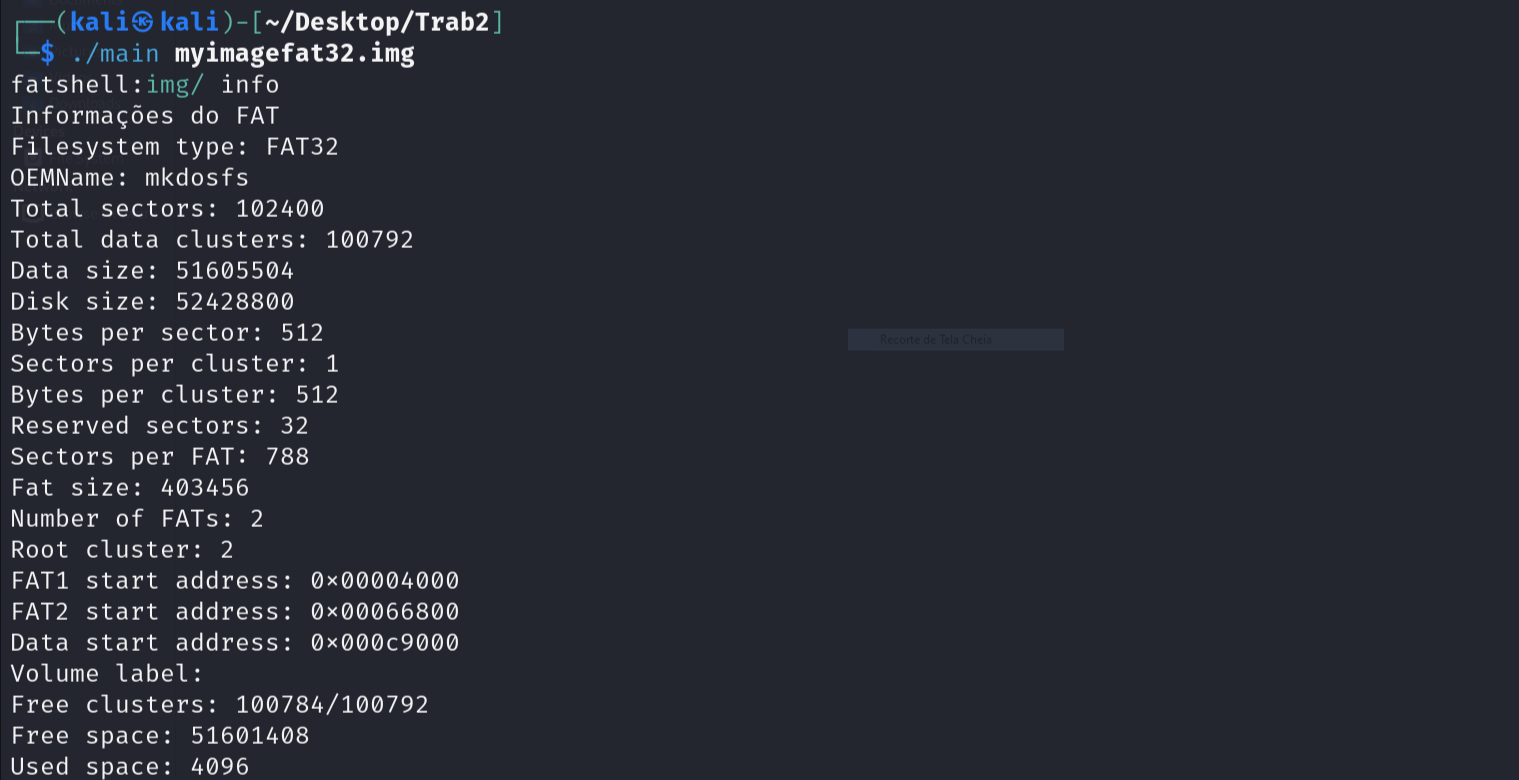
\includegraphics[width=450pt]{0-info.PNG}
    \caption{Saída do comando \texttt{info}}
    \label{fig:info}
\end{figure}

% --------------

\subsection{\texttt{ls}}
\label{subsec:ls}
Utilização: \$ \texttt{ls [caminho]} 

O comando \texttt{ls} lista os arquivos e diretórios do caminho atual ou do caminho descrito no primeiro parâmetro dele, a sua saída executada no caminho atual pode ser verificada na Figura~\ref{fig:ls}.

\begin{figure}[H]
    \centering
    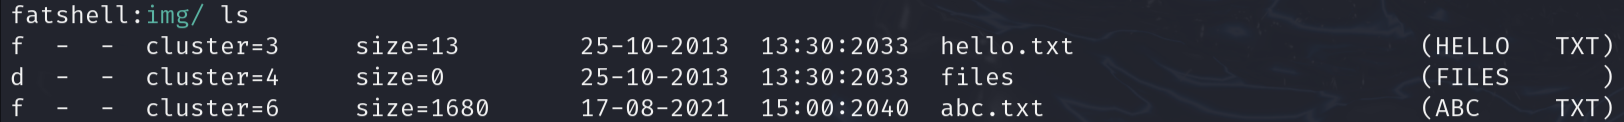
\includegraphics[width=450pt]{figuras/resultados/1-ls.PNG}
    \caption{Saída do comando \texttt{ls} executado no caminho atual}
    \label{fig:ls}
\end{figure}

% --------------

\subsection{\texttt{cluster}}
\label{subsec:cluster}
Utilização: \$ \texttt{cluster <número do cluster>}

O comando \texttt{cluster} exibe o conteúdo de um cluster em específico, exemplo de uso na Figura~\ref{fig:cluester}.

\begin{figure}[H]
    \centering
    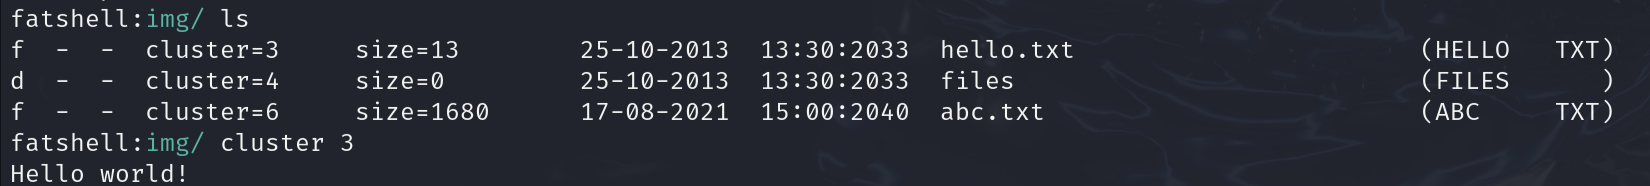
\includegraphics[width=450pt]{figuras/resultados/2-cluster.PNG}
    \caption{Saída do comando \texttt{cluster}}
    \label{fig:cluester}
\end{figure}

% --------------

\subsection{\texttt{cp}}
\label{subsec:cp}
Utilização: \$ \texttt{cp <origem> <destino>}  

O comando \texttt{cp} realiza a cópia de um arquivo do caminho de origem para o caminho de destino, podendo efetuar a cópia entre o sistema da imagem e o sistema de arquivo do host sistemas de arquivos ou dentro do próprio sistema da imagem. A cópia de um arquivo externo para o FAT32 pode ser verificada na Figura~\ref{fig:cp-externo-interno-1} e seu resultado na Figura~\ref{fig:cp-externo-interno-2}.

\begin{figure}[H]
    \centering
    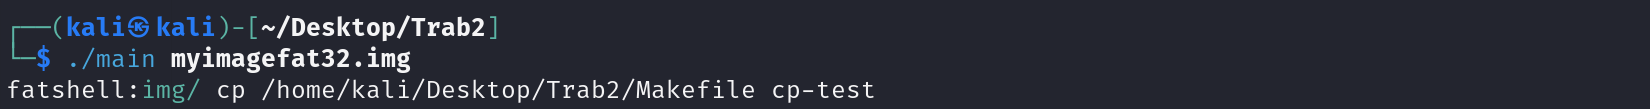
\includegraphics[width=450pt]{figuras/resultados/3.1-cp-externo-interno.PNG}
    \caption{Execução do comando \texttt{cp} para copiar arquivo externo para o FAT32}
    \label{fig:cp-externo-interno-1}
\end{figure}

\begin{figure}[H]
    \centering
    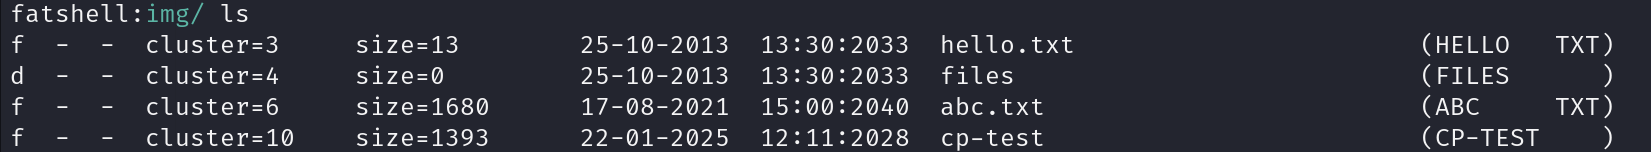
\includegraphics[width=450pt]{figuras/resultados/3.2-cp-externo-interno.PNG}
    \caption{Resultado da cópia do arquivo externo}
    \label{fig:cp-externo-interno-2}
\end{figure}

A cópia de um arquivo para o próprio FAT32 pode ser verificada na Figura~\ref{fig:cp-interno-attr}.

\begin{figure}[H]
    \centering
    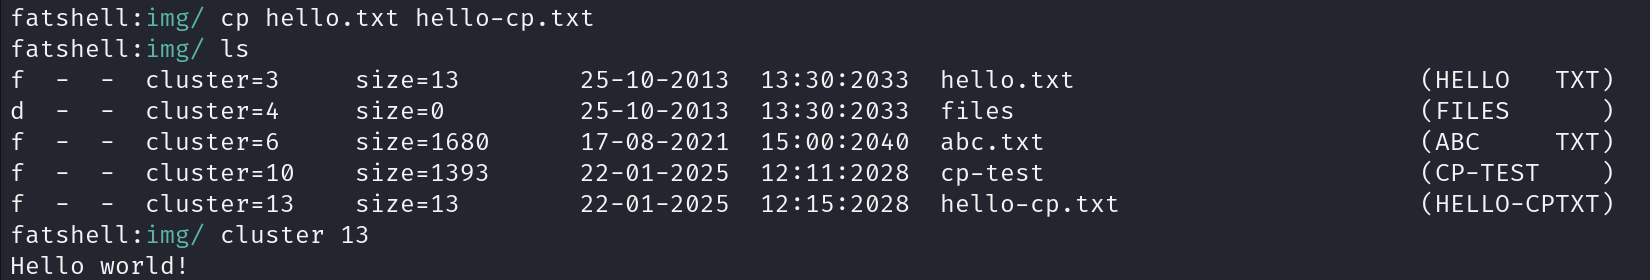
\includegraphics[width=450pt]{figuras/resultados/5-cp-interno-attr.PNG}
    \caption{Executação e resultado do comando \texttt{cp}, utilizado no próprio FAT32}
    \label{fig:cp-interno-attr}
\end{figure}

A cópia do arquivo residente no FAT32 para o sistema de arquivos externo pode ser verificada na Figura~\ref{fig:cp-interno-externo-1} e o seu resultado na Figura~\ref{fig:cp-interno-externo-2}.

\begin{figure}[H]
    \centering
    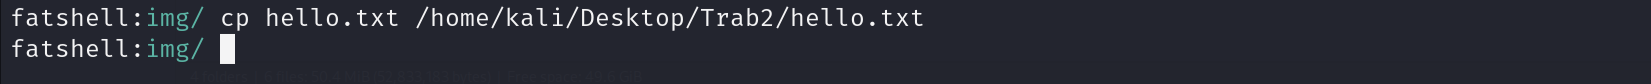
\includegraphics[width=450pt]{figuras/resultados/6-cp-interno-externo.PNG}
    \caption{Execução do comando \texttt{cp} realizando a cópia de um arquivo interno para o sistema de arquivos externo}
    \label{fig:cp-interno-externo-1}
\end{figure}

\begin{figure}[H]
    \centering
    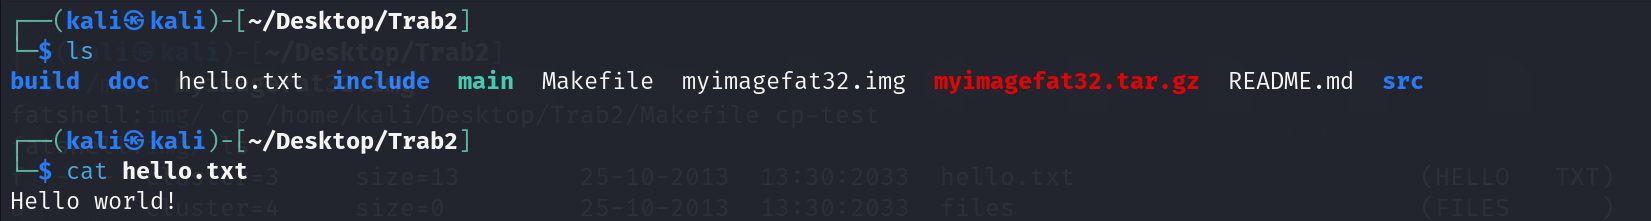
\includegraphics[width=450pt]{figuras/resultados/7-cp-arquivo-externo-resultado.PNG}
    \caption{Resultado no sistema de arquivos internos após cópia de arquivo resistente no FAT32}
    \label{fig:cp-interno-externo-2}
\end{figure}

% --------------

\subsection{\texttt{attr}}
\label{subsec:attr}
Utilização: \$ \texttt{attr <diretório | arquivo> }

O comando \texttt{attr} exibe os atributos de um arquivo ou diretório, a Figura~\ref{fig:attr} mostra a saída deste comando.

\begin{figure}[H]
    \centering
    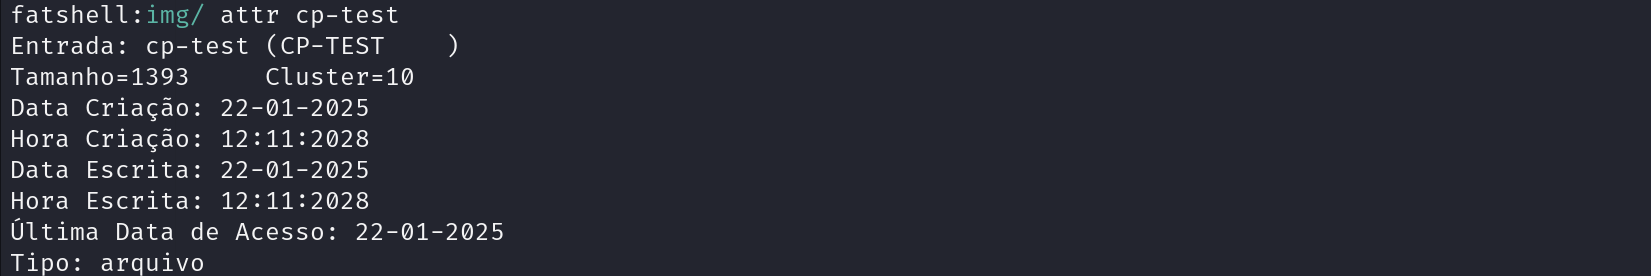
\includegraphics[width=450pt]{figuras/resultados/4-attr.PNG}
    \caption{Exemplo de saída para o comando \texttt{attr} utilizado em um arquivo}
    \label{fig:attr}
\end{figure}

% --------------

\subsection{\texttt{touch}}
\label{subsec:touch}
Utilização: \$ \texttt{touch} (nome)

O comando \texttt{touch} cria um arquivo sem conteúdo, a Figura~\ref{fig:touch} mostra a execução deste comando.

\begin{figure}[h!]
    \centering
    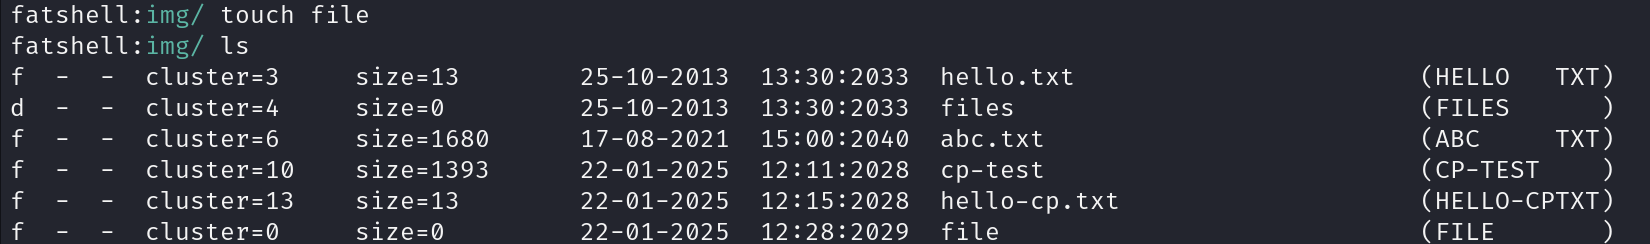
\includegraphics[width=450pt]{figuras/resultados/8-touch.PNG}
    \caption{Exemplo de uso do comando \texttt{touch}}
    \label{fig:touch}
\end{figure}

% --------------

\subsection{\texttt{mkdir}}
\label{subsec:mkdir}
Utilização: \$ \texttt{mkdir <nome>}

O comando \texttt{mkdir} cria um diretório vazio, um exemplo da sua utilização pode ser analisado na Figura~\ref{fig:mkdir}.

\begin{figure}[H]
    \centering
    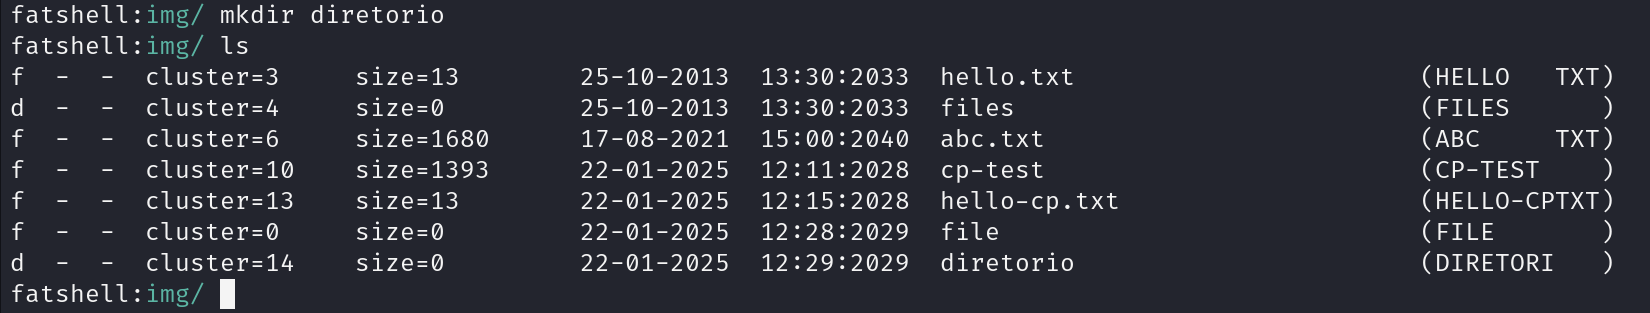
\includegraphics[width=450pt]{figuras/resultados/9-mkdir.PNG}
    \caption{Exemplo de uso do comando \texttt{mkdir}}
    \label{fig:mkdir}
\end{figure}

% --------------

\subsection{\texttt{cd}}
\label{subsec:cd}
Utilização: \$ \texttt{cd <destino>}

O comando \texttt{cd} possibilita navegar entre os diretórios, um exemplo da sua utilização pode ser analisado na Figura~\ref{fig:cd}.
 
\begin{figure}[H]
    \centering
    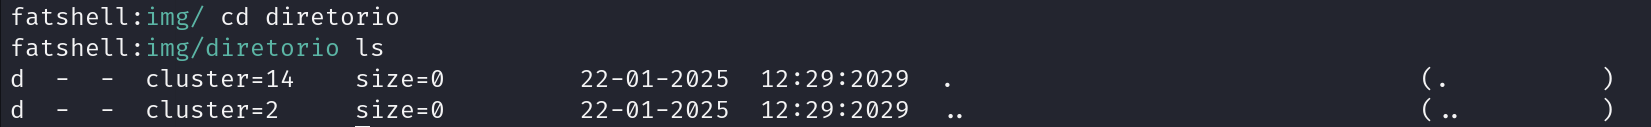
\includegraphics[width=450pt]{figuras/resultados/10-cd.PNG}
    \caption{Exemplo de utilização do comando \texttt{cd}}
    \label{fig:cd}
\end{figure}

% --------------

\subsection{\texttt{rename}}
\label{subsec:rename}
Utilização: \$ \texttt{rename <arquivo alvo> <arquivo com novo nome>}

O comando \texttt{rename} altera o nome de um arquivo específico, um exemplo da sua utilização pode ser analisado na Figura~\ref{fig:rename}.

\begin{figure}[H]
    \centering
    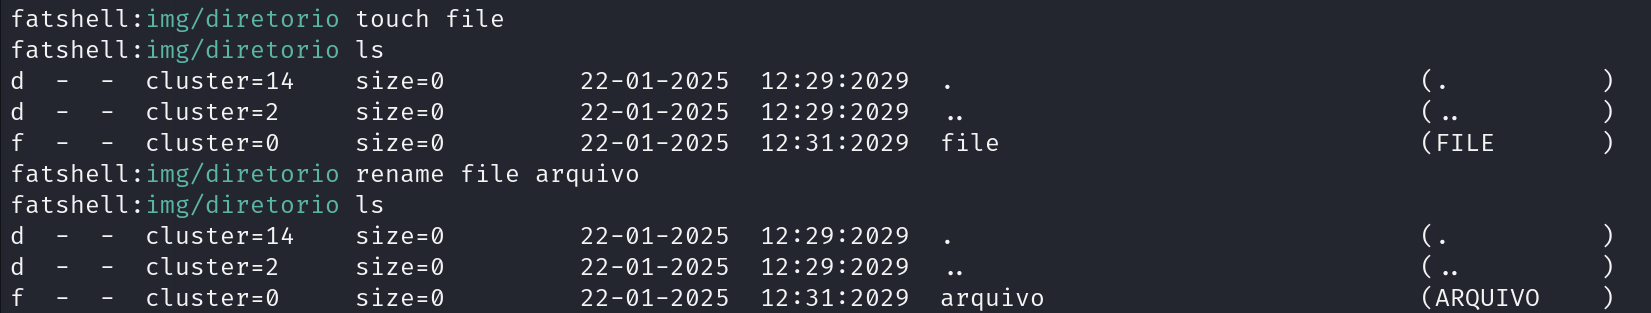
\includegraphics[width=450pt]{figuras/resultados/11-rename.PNG}
    \caption{Exemplo de utilização do comando \texttt{rename}}
    \label{fig:rename}
\end{figure}

% --------------

\subsection{\texttt{mv}}
\label{subsec:mv}
Utilização: \$ \texttt{mv <origem> <destino>}

O comando \texttt{mv} move arquivos para um destino específico, assim como o comando \texttt{cp} também pode ser usado para interagir com o sistema de arquivo original do sistema operacional, um exemplo da sua utilização movendo um arquivo do sistema de arquivos externo para o FAT32, pode ser analisado na Figura~\ref{subsec:mv}.

\begin{figure}[H]
    \centering
    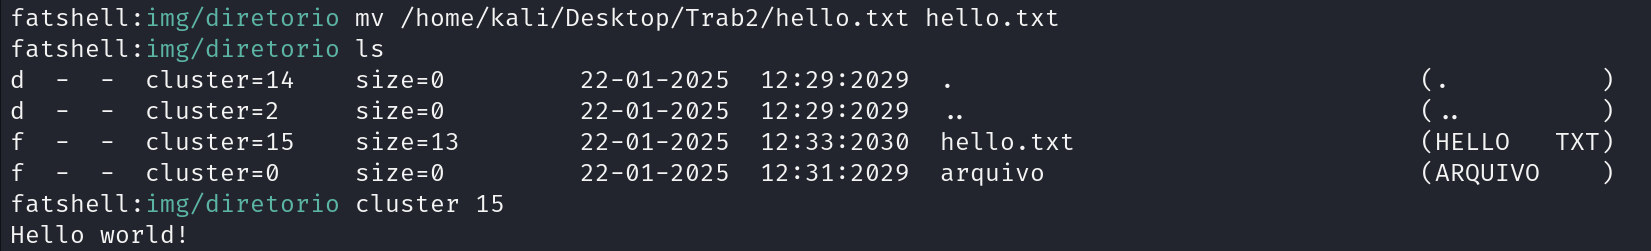
\includegraphics[width=450pt]{figuras/resultados/12-mv-externo-iterno.PNG}
    \caption{Exemplo do comando \texttt{mv} movendo arquivo externo para o FAT32}
    \label{fig:mv-externo-interno}
\end{figure}

O exemplo de mover um arquivo do FAT32 para o sistema de arquivos externo pode ser analisado na Figura~\ref{fig:mv-interno-externo} e sua validação na Figura~\ref{fig:mv-externo-validacao}.

\begin{figure}[H]
    \centering
    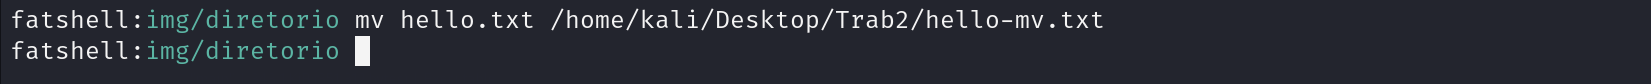
\includegraphics[width=450pt]{figuras/resultados/13-mv-interno-externo.PNG}
    \caption{Exemplo do comando \texttt{mv} movendo um arquivo do FAT32 para o sistema de arquivos externo}
    \label{fig:mv-interno-externo}
\end{figure}

\begin{figure}[H]
    \centering
    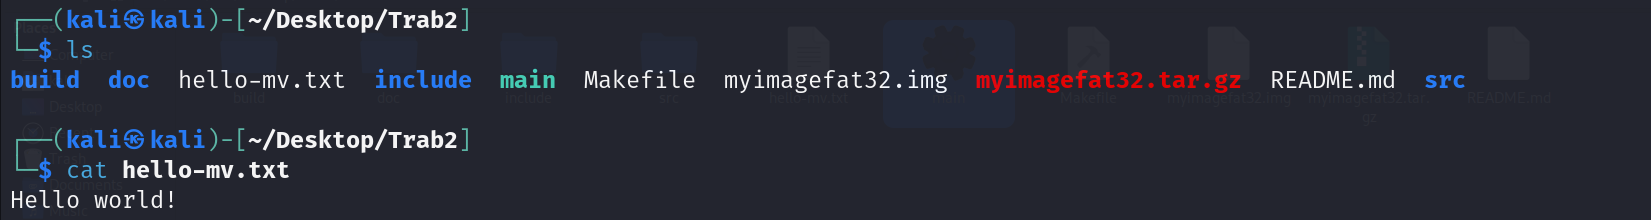
\includegraphics[width=450pt]{figuras/resultados/14-mv-externo-validacao.PNG}
    \caption{Resultado do comando \texttt{mv} movendo um arquivo do FAT32 para o sistema de arquivos externo}
    \label{fig:mv-externo-validacao}
\end{figure}

O exemplo de mover um arquivo interno para o próprio FAT32, pode ser verificado na Figura~\ref{fig:mv-interno}.

\begin{figure}[H]
    \centering
    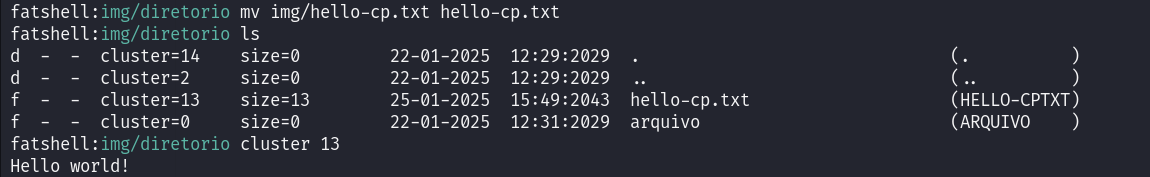
\includegraphics[width=450pt]{figuras/resultados/18-mv-interno-interno.PNG}
    \caption{Exemplo do comando \texttt{mv} movendo arquivo internamente no FAT32}
    \label{fig:mv-interno}
\end{figure}

% --------------

\subsection{\texttt{rm}}
\label{subsec:rm}
Utilização: \$ \texttt{rm <arquivo>}

O comando \texttt{rm} remove um arquivo em especifico do sistema de arquivos, um exemplo para sua utilização pode ser encontrado na Figura~\ref{fig:rm}.

\begin{figure}[H]
    \centering
    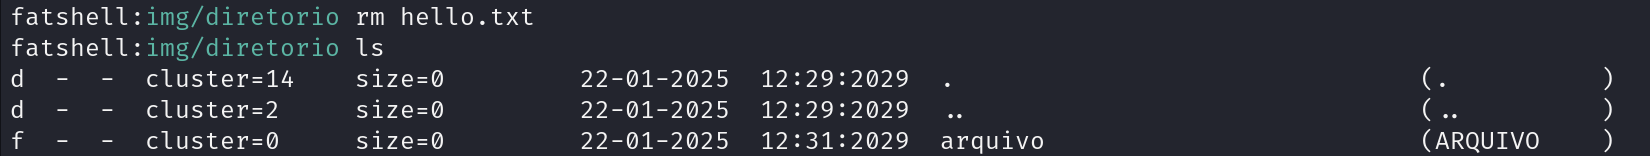
\includegraphics[width=450pt]{figuras/resultados/16-rm.PNG}
    \caption{Exemplo da utilização do comando \texttt{rm}}
    \label{fig:rm}
\end{figure}

% --------------

\subsection{\texttt{rmdir}}
\label{subsec:rmdir}
Utilização: \$ \texttt{rmdir <diretorio>}

O comando \texttt{rmdir} remove um diretório específico caso ele esteja vazio, um exemplo da sua utilização pode ser encontrado na Figura~\ref{fig:rmdir}.

\begin{figure}[H]
    \centering
    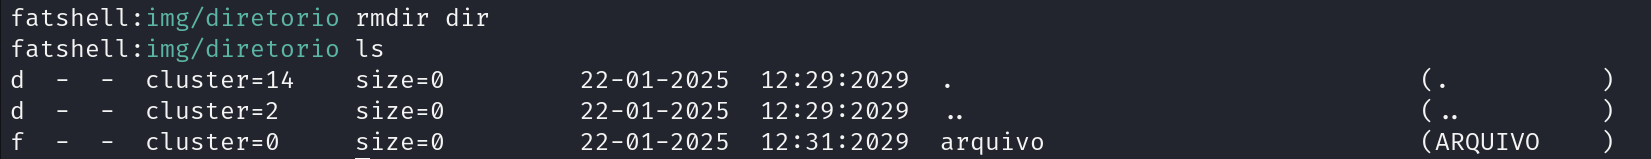
\includegraphics[width=450pt]{figuras/resultados/17-rmdir.PNG}
    \caption{Exemplo da utilização do comando \texttt{rmdir}}
    \label{fig:rmdir}
\end{figure}

% --------------

\subsection{\texttt{pwd}}
\label{subsec:pwd}
Utilização: \$ \texttt{pwd}

O comando \texttt{pwd} exibe o caminho absoluto atual, um exemplo da sua saída pode ser encontrado na Figura~\ref{fig:pwd}.

\begin{figure}[H]
    \centering
    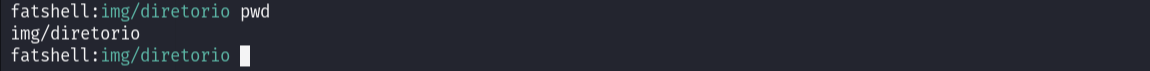
\includegraphics[width=450pt]{figuras/resultados/19-pwd.PNG}
    \caption{Exemplo da saída do comando \texttt{pwd}}
    \label{fig:pwd}
\end{figure}

% --------------

\section{Conclusões}
\label{sec:conclusoes}
A implementação do sistema de arquivos FAT32 permitiu consolidar conceitos teóricos sobre a organização e implementação de um sistema de arquivos, em especial o FAT32, destacando a sua organização de dados em disco, gerenciamento de metadados e alocação de clusters. A estrutura modular do código, dividida em componentes como tabela FAT, entradas de diretório e manipulação de imagens de disco, facilitou a manutenção e o teste individual de cada funcionalidade. O shell desenvolvido provou ser eficaz na interação com o sistema, executando comandos complexos como cópia entre sistemas de arquivos externos e internos, movimentação de arquivos e renomeação. Os principais desafios durante a implementação do sistema foi a manipulação de nomes longos e a garantia de integridade do sistema todo. Ainda assim, acreditamos que o resultado foi positivo, tanto para o nosso aprendizado quanto para o êxito do projeto em si.

% ----------------------------------------------------------
% ELEMENTOS PÓS-TEXTUAIS
% ----------------------------------------------------------
\postextual
% ----------------------------------------------------------
% Referências bibliográficas
% ----------------------------------------------------------
\renewcommand{\bibsection}{%
\section{\bibname}
\bibmark
%\ifnobibintoc\else
%\phantomsection
%\addcontentsline{toc}{section}{\bibname}
%\fi
\prebibhook}

\bibliography{abntex2-modelo-references}

\end{document}

